\documentclass[conference]{IEEEtran}
\IEEEoverridecommandlockouts
% The preceding line is only needed to identify funding in the first footnote. If that is unneeded, please comment it out.
\usepackage{cite}
\usepackage{hyperref}
\usepackage{amsmath,amssymb,amsfonts}
\usepackage{algorithmic}
\usepackage{graphicx}
\usepackage{subcaption}
\usepackage{textcomp}
\usepackage{xcolor}
\usepackage{geometry}
\usepackage{booktabs} % For professional looking tables
\usepackage{array}    % For table wrapping
\usepackage{tabularx}
\geometry{
top=1.9cm,
bottom=1.9cm,
left=0.8cm,
right=0.8cm,
columnsep=0.7cm
}

\def\BibTeX{{\rm B\kern-.05em{\sc i\kern-.025em b}\kern-.08em
    T\kern-.1667em\lower.7ex\hbox{E}\kern-.125emX}}
\begin{document}



\title{Deep Learning and Robotics\\
}

\author{\IEEEauthorblockN{Yongjiang Liu}}

\maketitle


%%%%%%%%%%%%%%%%%%%%%%%%%%%%%%%%%%%%%%%%%%%%%%%%%%%%%%%%%%
%Introduction && Overview
%%%%%%%%%%%%%%%%%%%%%%%%%%%%%%%%%%%%%%%%%%%%%%%%%%%%%%%%%%
\section{\textbf{State-of-the-Art in Robotics and Deep learning}}
With technological advancements, robotics remains a consistently popular research topic. Initially, robots were designed to perform simple, repetitive, and often hazardous tasks within controlled environments—for instance, Waldo~\cite{technovelgy_waldo} utilized in nuclear operations. Traditional robots heavily depended on hand-crafted, rule-based instructions and rigid pipelines, significantly limiting their adaptability to dynamic tasks and changing environments~\cite{brooks1991new}.

In the post-LLM era, robotics has evolved beyond mere automation toward the paradigm of embodied intelligence~\cite{roy2021machine}. Robots are now expected to operate effectively within unstructured and dynamic real-world environments and interact with humans naturally and collaboratively~\cite{licardo2024intelligent}. This evolution presents unique challenges absent from purely virtual AI settings, such as navigating physical uncertainties, grounding abstract concepts into tangible perception and actions, and learning effectively from sparse feedback~\cite{wang2024large}. Additionally, robots encounter substantial difficulty in comprehending real-world physical laws and aligning these understandings with their physical embodiments~\cite{liu2024aligning}.

Advancements in deep learning have significantly enhanced robotic capabilities by enabling effective learning from high-dimensional sensor data, thus allowing robots to acquire complex behaviors directly through deep imitation learning~\cite{levine2016end}. However, imitation learning approaches are notably data-intensive. To address this limitation, transfer learning techniques have emerged as practical solutions for fine-tuning pretrained models, significantly reducing the demand for extensive real-world data collection. Moreover, recent developments in deep reinforcement learning (DRL) provide promising methodologies to further fine-tune end-to-end trained robotic models by enabling interactive adaptation within specific real-world scenarios~\cite{tang2024deep}.

As research progresses, Cognitive Robotics—which intersects robotics, developmental psychology, and biology—has drawn significant attention. Researchers envision cognitive robots capable of self-driven development analogous to human cognitive evolution, continually enhancing their understanding of the world through perception, interaction, and embodied experiences~\cite{cangelosi2015developmental}. The expectation is to leverage contemporary artificial intelligence methodologies to impart these cognitive capacities to robots~\cite{brooks1991intelligence}. In the following sections, We will critically review current developments concerning perception, motion, interaction, and their associated limitations.

\subsection{Perception: Deep Learning for Embodied Visual Cognition}
Perception forms the foundational basis for intelligent robotic behavior, enabling robots to interpret, respond to, and interact effectively with their environments. Unlike human vision, where visual information passes sequentially through the cornea, pupil, lens, vitreous body, and finally focuses onto the retina, robots initially relied on traditional computer vision (CV) methods, such as SIFT and other rule-based approaches. These conventional pipelines, characterized by hand-crafted features and deterministic rules, often proved inadequate in noisy or dynamically changing scenarios~\cite{o2020deep}.

With advancements in deep learning, robots gained the ability to learn hierarchical representations directly from raw sensory inputs. From early architectures like LeNet~\cite{lecun1998gradient}, capable of recognizing simple digits, to AlexNet~\cite{krizhevsky2012imagenet} and subsequently deeper architectures such as VGG~\cite{simonyan2014very}, convolutional neural networks (CNNs) progressively improved in both classification accuracy and generalization capabilities. However, CNN architectures faced limitations in increasing depth until the introduction of ResNet, which fundamentally transformed the landscape through residual connections, enabling significantly deeper and more accurate models~\cite{he2016deep}.

Further advancements in object detection frameworks, such as YOLO~\cite{jiang2022review} and Mask R-CNN~\cite{bharati2020deep}, extended robotic perception capabilities by providing real-time localization, object tracking, and instance segmentation, crucial for spatial understanding and interaction with dynamic environments.

For more sophisticated scene comprehension, Graph Neural Networks (GNNs) emerged as a powerful tool, effectively modeling the spatial layout and inter-object relationships by treating detected entities as nodes within graph structures~\cite{lin2022efficient}. This capability is particularly advantageous for robotic tasks involving grasp planning in cluttered or unstructured environments.

Recently, Vision Transformers (ViT) introduced a global attention-based modeling approach, enabling robots to capture long-range dependencies within visual data, enhancing robustness against noise, occlusions, and domain shifts~\cite{dosovitskiy2020image}. Techniques such as DINOv2 have further extended these capabilities, providing advanced solutions for image matching, segmentation, and depth estimation~\cite{oquab2023dinov2}.

Ensuring precise, error-free environmental understanding represents a critical first step toward achieving truly cognitive robotics. Cognitive robotics aims for robots not merely to perceive but to build a continuous and dynamic understanding through embodied interaction and experiential learning. In essence, the integration of cutting-edge perception methods—ranging from CNNs and GNNs to Vision Transformers—marks an essential milestone in equipping robots with cognitive abilities paralleling human-level adaptability, resilience, and intelligent decision-making.

\subsection{Motion: Learning to Act in Dynamic Environments}

Beyond perception, cognitive robots must purposefully act within their environments. Motion involves not merely executing predefined trajectories but dynamically adapting behaviors based on real-time sensory inputs and goal-oriented reasoning. Thus, motion represents a critical aspect of embodied cognition, reflecting a continuous perception-action feedback loop.

A fundamental technique facilitating this capability is Simultaneous Localization and Mapping (SLAM), which enables robots to construct spatial maps while simultaneously localizing themselves. Variants like visual SLAM (vSLAM)~\cite{grisetti2010tutorial} and biologically-inspired methods such as RatSLAM leverage visual inputs alongside neural models of spatial memory, enhancing navigation robustness and cognitive plausibility~\cite{milford2004ratslam}.

Beyond localization, effective robotic motion requires trajectory planning and execution that consider obstacle avoidance, balance maintenance, and task objectives. Reinforcement Learning (RL) has emerged as a potent solution to address these challenges~\cite{kormushev2013reinforcement}. Algorithms such as Proximal Policy Optimization (PPO)~\cite{schulman2017proximal}, Soft Actor-Critic (SAC)~\cite{haarnoja2018soft}, and Deep Deterministic Policy Gradient (DDPG)~\cite{qiu2019deep} allow robots to learn motor policies via iterative interaction and trial-and-error processes, optimizing cumulative rewards. This approach facilitates generalized behavior without the necessity of explicit instruction. Additionally, self-calibration techniques further refine motion by continuously adjusting actuator alignments and joint coordination using visual feedback~\cite{fang2022self}. Such sensorimotor coupling epitomizes the embodied learning paradigm, supporting lifelong learning and autonomous adaptation~\cite{bahadir2023investigating}.

\subsection{Interaction: Human-Robot Collaboration}
Effective social interaction differentiates cognitive robots from traditional task-oriented robotic systems. In fields such as education, healthcare, and domestic assistance, robots must accurately interpret and respond to sophisticated social signals, including gestures, speech, facial expressions, and emotional states~\cite{cangelosi2022cognitive}. This multimodal interaction demands temporally coherent and contextually aware models capable of sophisticated social cognition~\cite{wake2024gpt}.

Language-based interaction capabilities have advanced notably through Large Language Models (LLMs), such as BERT~\cite{devlin2019bert} and GPT~\cite{radford2018improving}, enabling robots to conduct coherent, goal-oriented conversations. Integrated with perception systems, these models facilitate grounded language understanding by associating verbal instructions with tangible objects and actionable tasks. For example, robots can accurately interpret and execute commands like "pick up the red cup next to the book" through multimodal reasoning.

Furthermore, Reinforcement Learning with Human Feedback (RLHF) enables robots to align their actions with human preferences, integrating subjective feedback directly into policy optimization~\cite{lin2020review}. Concurrently, imitation learning supports social skill acquisition by allowing robots to observe and replicate human actions, aligning with developmental learning principles of continuous skill evolution.

\section{Methodology}
\subsection{Classification Principle}
Deep Neural Networks (DNNs) are widely employed for image classification tasks. The primary objective is to learn a non-linear function \( f(\mathbf{x}; \theta) \) that maps an input image \( \mathbf{x} \in \mathbb{R}^d \) to one of \( C \) discrete class labels. The network produces a probability distribution over classes via the softmax function applied to the logits from its final layer:

\[
\hat{y}_i = \frac{e^{z_i}}{\sum_{j=1}^{C} e^{z_j}}
\]

The predicted label corresponds to the class with the highest probability in the vector \( \hat{\mathbf{y}} \). This approach enables end-to-end optimization using gradient-based training.

\subsection{Dataset Description}
We use the CIFAR-100 dataset for our experiments, which comprises 60{,}000 color images of size \(32 \times 32\) pixels, evenly distributed across 100 distinct classes with 600 images per class~\cite{krizhevsky2009learning}.

The choice of CIFAR-100 is further justified by contrasting it with alternative datasets. CIFAR-10 lacks sufficient class granularity; MNIST is limited by its grayscale format and low visual complexity; ImageNet exceeds the scope of our available computational resources; and MS-COCO is designed for object detection rather than classification. Therefore, CIFAR-100 provides a suitable balance between complexity and feasibility, making it an ideal benchmark for exploring architectural properties of models such as ResNet and ViT within our experimental constraints. Its high intra-class variability and fine-grained class distinctions also make it particularly effective for evaluating model robustness under input perturbations.
\subsection{Model Architectures}
We compare two deep learning architectures: ResNet (a Convolutional Neural Network) and ViT-B/16 (a Transformer-based vision model). ResNet architectures are trained from scratch on CIFAR-100 using a Weights \& Biases (W\&B) sweep for hyperparameter optimization. In contrast, ViT-B/16 is pretrained on ImageNet-21k and subsequently fine-tuned on the CIFAR-100 dataset.

ResNet introduces \textit{residual connections} to address the degradation problem in deep networks by enabling identity mappings across layers. Each residual block applies convolutional transformations followed by a skip connection, which adds the input directly to the output:
\[
\mathbf{y} = \mathcal{F}(\mathbf{x}) + \mathbf{x},
\]
where \( \mathcal{F}(\mathbf{x}) \) denotes the residual mapping. This structure facilitates gradient flow, stabilizes training, and allows effective optimization of very deep networks. In our setting, CIFAR-100 images (\(32\times32\times3\)) are first passed through a \(3\times3\) convolution and then through four stages of residual blocks.

\textbf{ViT-B/16.} Vision Transformer (ViT) applies a transformer architecture directly to image patches. Each input image is split into \(16\times16\) non-overlapping patches and linearly projected into embeddings. A learnable \texttt{[CLS]} token is prepended to the patch sequence and positional embeddings are added. The sequence is processed through multiple self-attention layers (transformer encoder), and the output corresponding to the \texttt{[CLS]} token is fed into an MLP head for classification.

Simpler architectures such as MLP, LeNet, AlexNet were excluded due to their shallow depth, absence of modern regularization mechanisms, and poor performance on large-scale image benchmarks. In particular, MLPs lack spatial inductive biases; LeNet and AlexNet are outdated; and VGG, while deep, is computationally inefficient without residual connections or attention mechanisms.

\subsection{Hyperparameter and Evaluation Setup}

We conduct systematic hyperparameter exploration to optimize model performance and ensure fair comparison between CNN-based and Transformer-based architectures.

\paragraph{ResNet Training.} ResNet models (ResNet18, ResNet34, ResNet50, ResNet101) are trained from scratch on CIFAR-100 using various hyperparameter configurations. The tested batch sizes include 16, 32, and 64; initial learning rates range from 0.005 to 0.1; and weight decay values are chosen between 5e-4 and 1e-2. Both SGD and AdamW optimizers are considered to evaluate optimization dynamics under different regularization strengths(Table~\ref{tab:hyperparameters_resnet}).

\paragraph{ViT Fine-Tuning.} For ViT experiments, we use the ViT-B/16 architecture pretrained on ImageNet-21k. Fine-tuning is performed on CIFAR-100 with batch sizes of 16, 32, and 64; learning rates ranging from 1e-4 to 5e-4; and weight decay values from 5e-4 to 1e-2. Both SGD and AdamW optimizers are tested, with AdamW generally preferred due to its compatibility with pre-trained transformer weights(Table~\ref{tab:hyperparameters_ViT}). The codebase for all experiments and evaluation in this project is available at the following GitHub repository\footnote{\url{https://github.com/yongjiangliu-uom/cider-100.git}}.


\begin{table}[!h]
\centering
\caption{Hyperparameter configurations for ResNet}
\label{tab:hyperparameters_resnet}
\begin{tabular}{@{}lc@{}}
\toprule
\toprule
\textbf{Hyperparameter} & \textbf{Values Tested} \\
\midrule
Architecture & ResNet18, ResNet34, ResNet50, ResNet101 \\
Batch Size & 16, 32, 64 \\
Initial Learning Rate & 0.005 to 0.1 \\
Weight Decay & 5e-4 to 1e-2 \\
Optimizer & SGD, AdamW \\
\bottomrule
\bottomrule
\end{tabular}
\end{table}

\subsubsection{Pretrained \texttt{ViT-B/16} Experiment Configuration}

\begin{table}[!h]
\centering
\caption{Hyperparameter configurations ViT}
\label{tab:hyperparameters_ViT}
\begin{tabular}{@{}lc@{}}
\toprule
\toprule
\textbf{Hyperparameter} & \textbf{Values Tested} \\
\midrule
Batch Size & 16, 32, 64 \\
Initial Learning Rate & 1e-4 to 5e-4 \\
Weight Decay & 5e-4 to 1e-2 \\
Optimizer & SGD, AdamW \\
\bottomrule
\bottomrule
\end{tabular}
\end{table}

\section{Result Analysis}
\begin{figure}[!h]
    \centering
    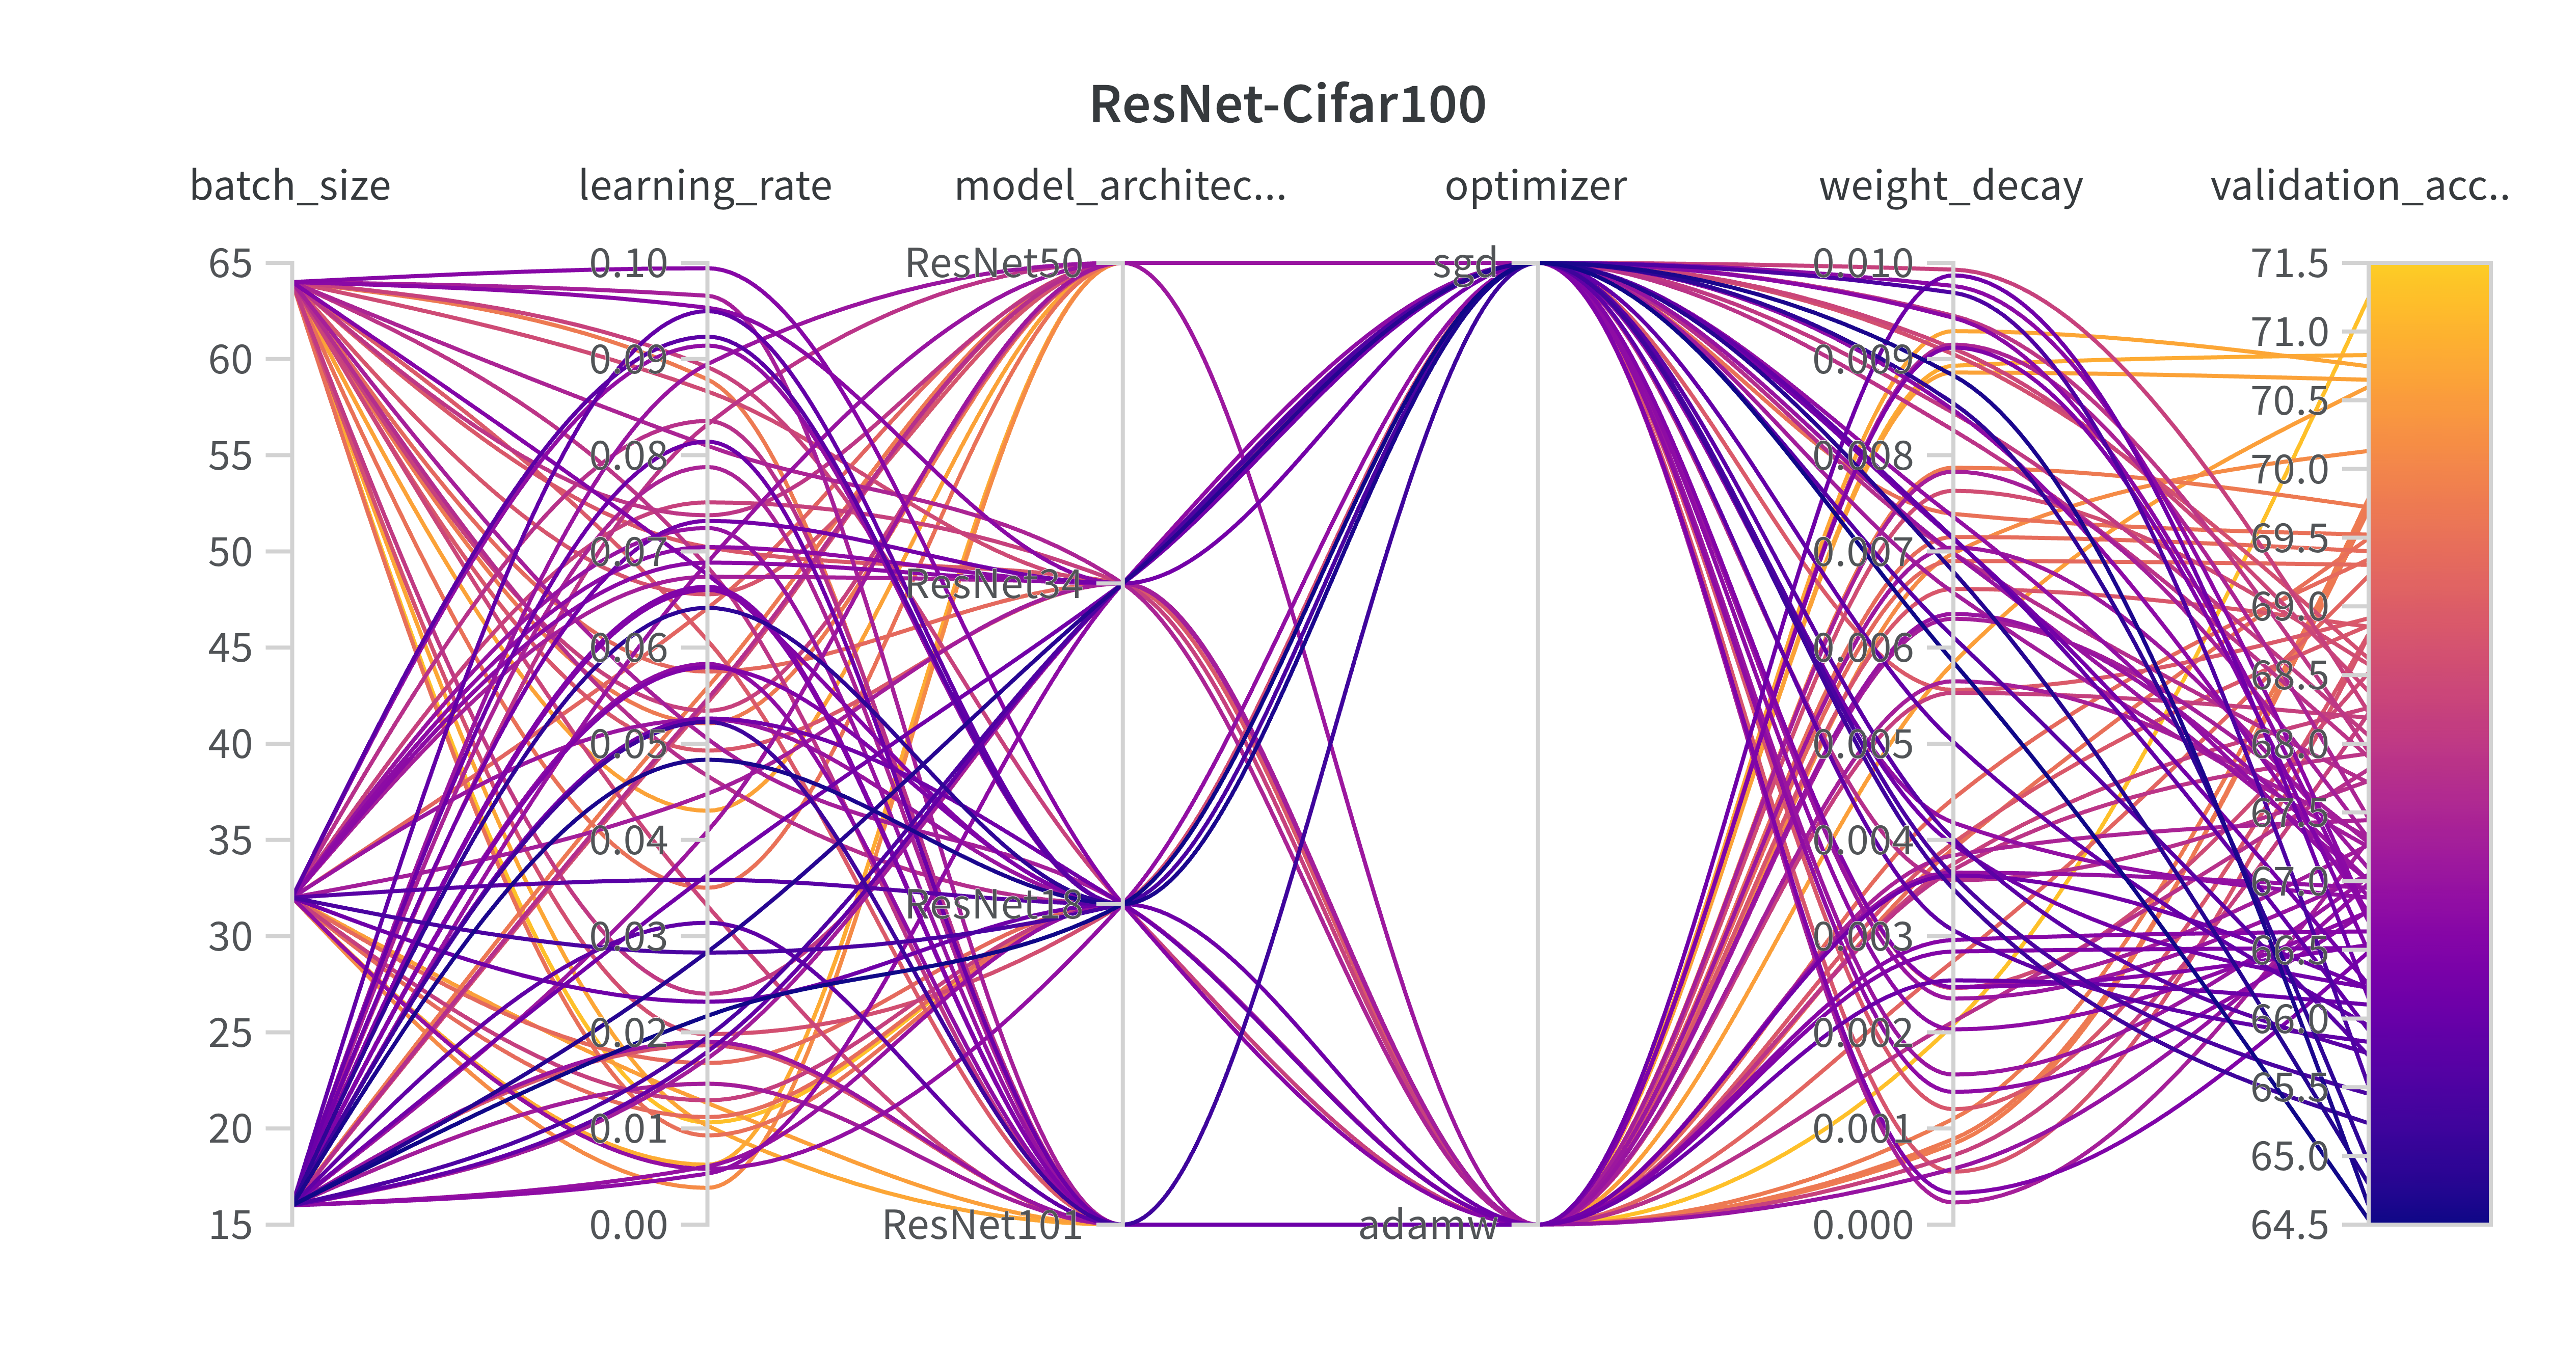
\includegraphics[width=0.6\linewidth]{resnet_wandb.png}
    \caption{Parallel coordinates plot for ResNet}
    \label{fig:resnet_hp_search}
\end{figure}

\begin{figure}[!h]
    \centering
    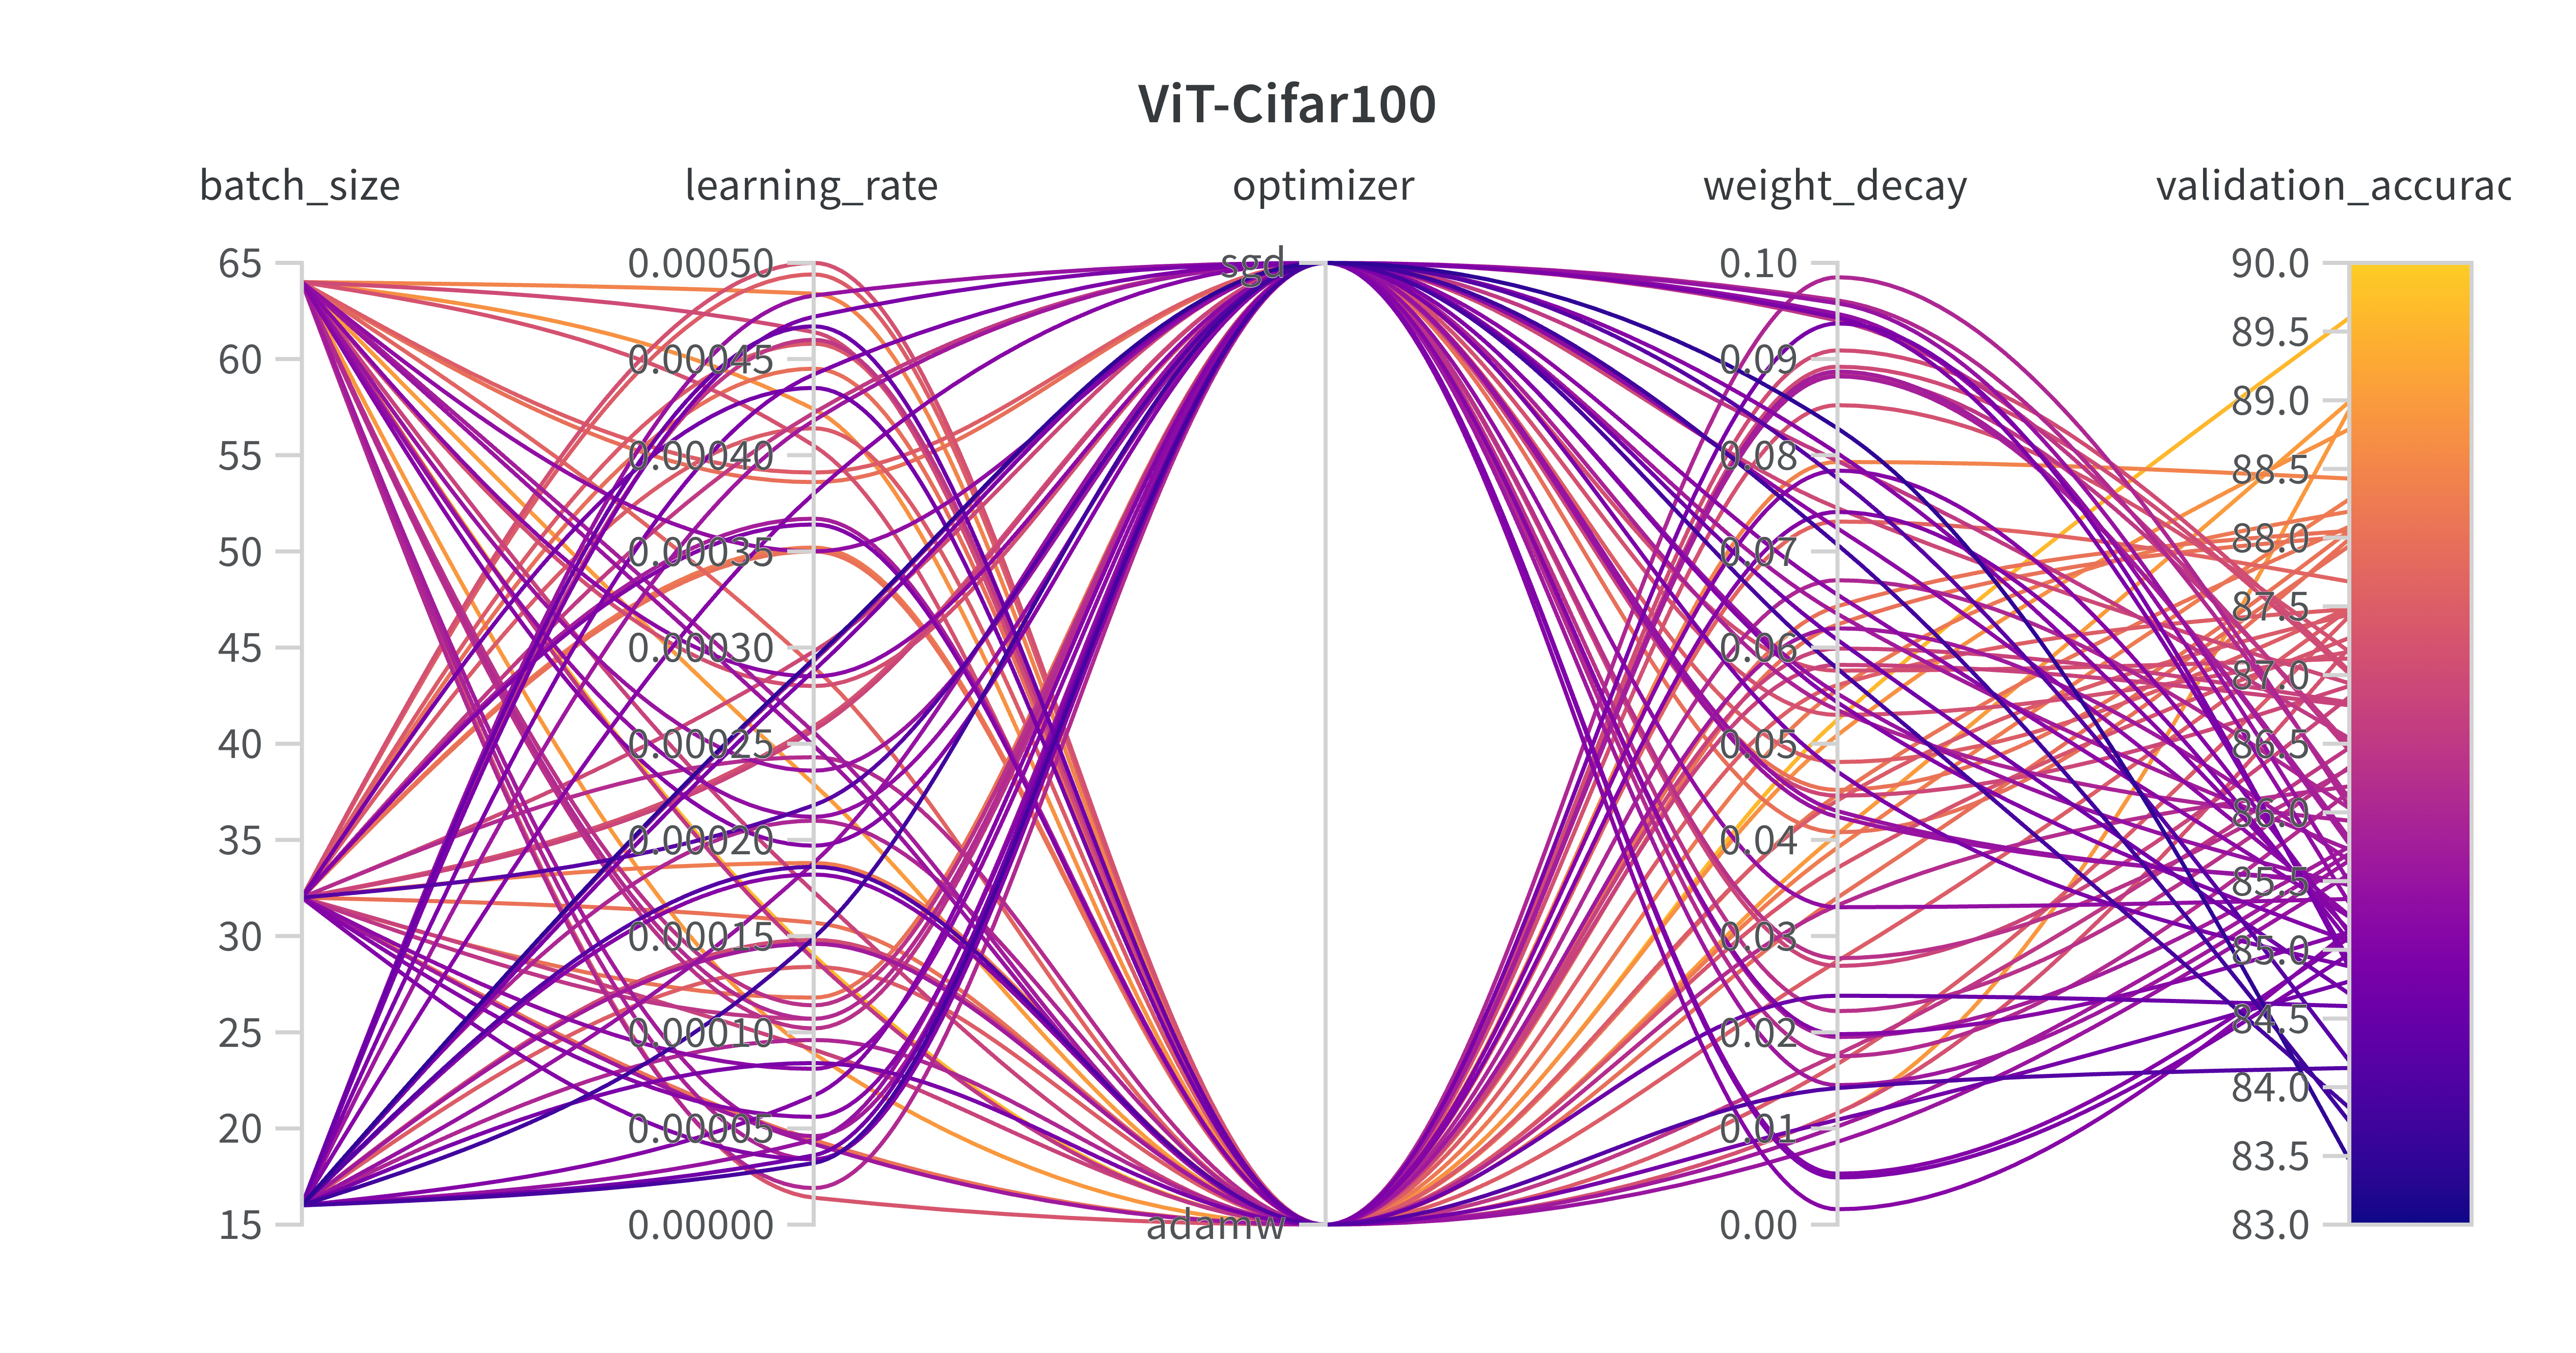
\includegraphics[width=0.6\linewidth]{vit_wandb.png}
    \caption{Parallel coordinates plot for ViT-B/16}
    \label{fig:vit_hp_search}
\end{figure}

\begin{table}[h]
\centering
\caption{ResNet Result}
\label{tab:resnet_details}
\begin{tabular}{@{}lcccr@{}} % Alignment: left, center, center, center, right
\toprule
\toprule
\textbf{Architecture} & \textbf{Batch Size} & \textbf{Dataset} & \textbf{Param No.} & \textbf{Top-1 Acc(\%)} \\ 
\midrule
ResNet18    & 64 & Cifar100 & 11.22M & 67.86\\
ResNet34    & 64 & Cifar100 & 21.33M & 68.64 \\
ResNet50    & 64 & Cifar100 & 23.71M & 70.81 \\
\textbf{ResNet101}   & \textbf{64} & \textbf{Cifar100} & \textbf{42.70M} & \textbf{71.48} \\
\textbf{ResNet50-PreTrain} & \textbf{64} & \textbf{Cifar100} & \textbf{23.71M} & \textbf{84.60} \\
\bottomrule
\bottomrule
\end{tabular}
\end{table}

\begin{table}[!h]
\centering
\caption{Model Performance (Top-1 Accuracy)}
\label{tab:model_performance}
\begin{tabular}{@{}llc@{}}
\toprule
\toprule
\textbf{Model} & \textbf{Image Resolution} & \textbf{Top-1 Acc. (\%)} \\
\midrule
ViT\_B\_16-Pretrain & 224×224 & 87.23 \\
\textbf{ViT\_B\_16 (official)} \cite{dosovitskiy2020image} & \textbf{384×384} & \textbf{94.2} \\
DeiT (official) \cite{touvron2021training} & 384×384 & 90.8 \\
\bottomrule
\bottomrule
\end{tabular}
\end{table}

\begin{figure}[!h]
    \centering
    \begin{minipage}[b]{0.22\textwidth}
        \centering
        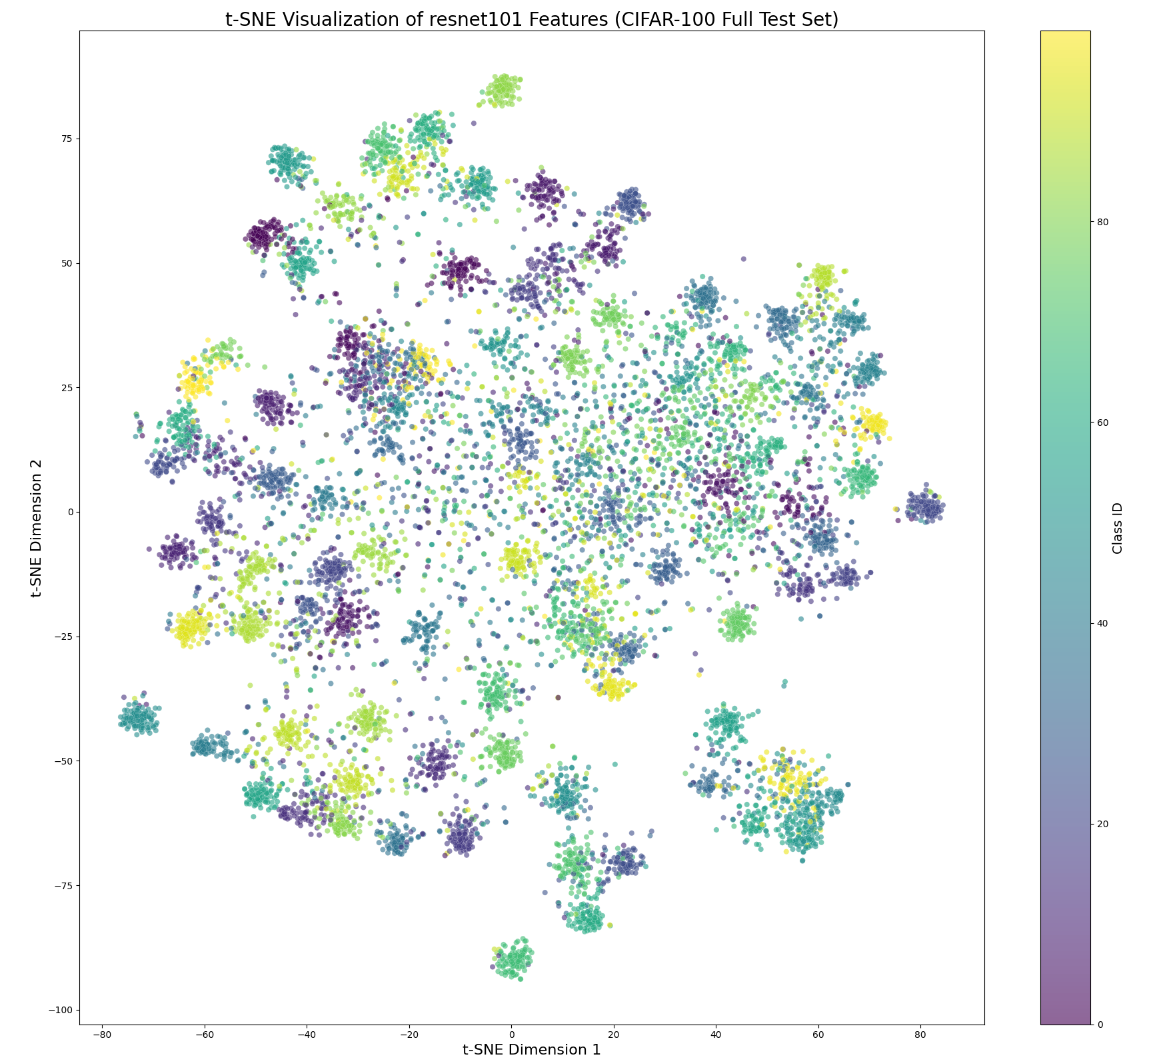
\includegraphics[width=\textwidth]{resnetv.png}
        \caption*{ResNet50}
    \end{minipage}
    \hfill
    \begin{minipage}[b]{0.22\textwidth}
        \centering
        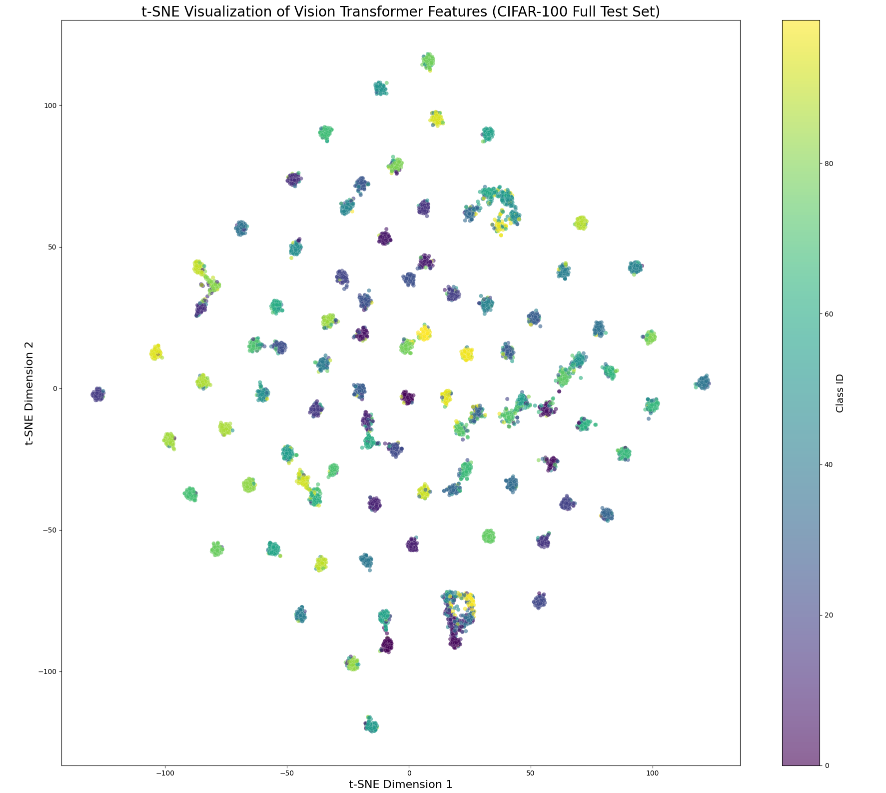
\includegraphics[width=\textwidth]{vitv.png}
        \caption*{ViT-B/16}
    \end{minipage}
    \caption{t-SNE visualization of feature embeddings}
    \label{fig:tsne_compare}
\end{figure}

Table~\ref{tab:resnet_details} and Table~\ref{tab:model_performance} provide a comparative analysis of ResNet and ViT architectures in terms of classification accuracy and model configuration. Within the ResNet family, we observed a clear trend of performance improvement with increased network depth: ResNet18 achieves a Top-1 accuracy of 67.86\% on CIFAR-100, while ResNet50 and ResNet101 attain 70.81\% and 71.48\%, respectively. However, the marginal gain from ResNet50 to ResNet101—despite a substantial increase in parameter count—suggests diminishing returns in performance when training deeper convolutional networks from scratch. Notably, applying ImageNet-21k pretraining to ResNet50 results in a significant boost to 84.60\%, which shows the importance of transfer learning for data-limited target tasks.

In comparison, the Vision Transformer ViT-B/16, pretrained on ImageNet-21k, achieves 87.23\% accuracy at a lower input resolution (224×224), outperforming all ResNet variants, including the pretrained ResNet50. Officially reported results for ViT-B/16 and DeiT at 384×384 resolution further push the performance boundary to 94.2\% and 90.8\%, respectively, highlighting the scalability and superior representational power of Transformer-based models under large-scale pretraining and higher input fidelity. The observed performance gap between our implementation and the official ViT benchmarks may be partially attributed to the reduced input resolution (224×224 vs. 384×384), which limits the spatial detail available to the self-attention mechanism. Since Transformer architectures lack strong spatial inductive biases, their performance is more sensitive to image resolution compared to convolutional models. This suggests that higher-resolution inputs are crucial for fully leveraging the capacity of ViT models in fine-grained classification tasks like CIFAR-100.

In summary, ViT-B/16 demonstrates consistently stronger performance. Pretraining method proves essential for both model families, and deeper CNNs exhibit saturation effects absent in Transformer architectures. These trends suggest that Transformers, while initially data-hungry, generalize more effectively when pretrained on large datasets. This conclusion is further supported by the t-SNE visualizations in Figure~\ref{fig:tsne_compare}, where ViT-B/16 exhibits more compact and well-separated clusters than ResNet50.


\section{Discussion}
While MLPs, ResNets, and Vision Transformers (ViTs) all employ similar final classification heads—typically a fully connected layer followed by a softmax function—their performance differs significantly due to the nature of their feature extractors. The core distinction lies not in the output classifier but in the way each architecture encodes input data into high-level representations.

Standard MLPs operate on flattened image vectors and lack any architectural bias toward the spatial structure inherent in visual data. Consequently, they are prone to overfitting, and perform poorly on complex image tasks. In contrast, ResNets employ convolutional layers with local receptive fields which capturing hierarchical spatial features such as edges, textures, and object contours. Residual connections further enhance the stability of training deep networks, enabling effective gradient flow and deeper representations.

ViT partition input images into fixed-size patches and model pairwise relationships between patches using self-attention. Unlike CNNs, ViTs lack strong spatial inductive biases, allowing them to model long-range dependencies and semantic context more effectively—provided sufficient pretraining on large-scale datasets. This global modeling capability grants ViTs robustness against certain types of noise and occlusion, but it also makes them more data-hungry and less effective when training data is limited~\cite{park2022vision}.

\section{Conclusion}
This study presents a comparative evaluation of two prominent deep learning architectures—ResNet and ViT-B/16—for image classification and robustness using the CIFAR-100 dataset. Despite both models sharing a standard MLP classification head, their underlying feature extraction mechanisms—convolutional for ResNet and self attention for ViT—led to markedly different performance~\cite{wu2022tinyvit}.

ResNet, equipped with strong spatial inductive biases through convolutional layers and residual connections, demonstrated stable performance. However, the pre-trained ViT-B/16 exhibited significantly higher performs better. These results highlight the superior generalization capacity of Transformer-based models when fine-tuned from large-scale pretraining~\cite{mauricio2023comparing}.

The implications of these findings are especially relevant for cognitive robotics, where perceptual robustness is critical for long-term autonomy, real-world interaction, and safe human collaboration. A robot’s ability to operate under sensor noise, partial observability, and dynamic lighting conditions fundamentally depends on the strength and adaptability of its perceptual subsystem. Vision Transformers, with their global modeling capabilities and data-driven representations, present a compelling foundation for next-generation embodied agents capable of functioning in open, unpredictable environments.

\subsection{Future Work}
Building on the experimental findings in this report, future work will involve manually implementing a ViT architecture from scratch in PyTorch and training it without pre-initialised weights. This will provide direct insights into the optimization dynamics, convergence challenges, and inductive biases (or lack thereof) associated with ViT when trained from limited data like CIFAR-100. Eventually, We will use the similar parameter's Resnet and ViT(both trained on the same dataset)to conduct the fair comparisons.

While ViT models demonstrate strong accuracy, several challenges remain to be addressed before they can be feasibly deployed in real-world robotic platforms. First, the ViT-B/16 model is computationally expensive and memory-intensive, making it unsuitable for many low-power robotic systems. Future work will explore lightweight Vision Transformers such as \textit{MobileViT}~\cite{mehta2021mobilevit}, \textit{TinyViT}~\cite{wu2022tinyvit}, and \textit{DeiT}~\cite{touvron2021training}, which aim to reduce model complexity while retaining rich representational capacity. In parallel, model compression techniques—such as quantisation, pruning, and neural architecture search (NAS)—will be studied to reduce inference latency and enable deployment on resource-constrained edge devices.

Second, real-world robotic agents must continuously adapt to novel tasks, evolving environments, and non-stationary sensor inputs. To this end, future research will investigate \textit{continual learning} and \textit{online adaptation} strategies. These methods align with core principles of cognitive robotics such as lifelong learning, knowledge adaptation, and situated perception-action coupling, and will be critical in enabling autonomous agents to operate robustly and adaptively in open-ended learning results.

\newpage
\bibliography{references.bib}
\bibliographystyle{unsrt}


\end{document}
